%Introduction chapitre III : Simulation

Ce chapitre présente $D^2CTS$ : un simulateur de terminal portuaire à conteneurs conçu et développé durant cette thèse. Les problèmes d'ordonnancement et d'affectation ainsi que de routage dynamique sont des problématiques théoriques ici inscrites dans un contexte concret. Les terminaux portuaires à conteneurs sont des structures privées difficilement abordables. Ils fonctionnent en continu et il est donc impossible de procéder à des tests grandeur nature sur une journée d'exploitation. Un simulateur permet ainsi de réaliser ces mesures de performance dans un environnement virtuel le plus réaliste possible avant d'hypothétiquement passer à la mise en place à l'échelle réelle. 

Le programme a été élaboré lors de la participation du LITIS au projet CALAS qui est l'acronyme de \textit{CArrier LAser tracking System}. Le projet consiste à élaborer une technologie de localisation des engins de manutention capable de fonctionner à n'importe quel endroit du terminal. En effet, la technologie de géolocalisation actuelle utilise des satellites (GPS : \textit{Global Positioning System}%TODO CHECK
) afin de déterminer les coordonnées d'un émetteur. Or, le signal des satellites traversant mal le métal, les véhicules qui se trouvent sous les portiques de déchargement ou dans les travées de conteneurs ne sont pas repérés.

La société \textit{Laser Data Technology Terminal} (LDTT) a mis au point une technologie de géolocalisation utilisant un rayon laser et exploitant la caractéristique physique principale des chariots cavaliers : leur hauteur. En effet, les chariots cavaliers sont les engins mobiles autonomes les plus élevés du terminal. Il est donc possible de déterminer leur position grâce à un signal horizontal émis à la hauteur du sommet des chariots cavaliers afin d'être en mesure de localiser les véhicules équipés à n'importe quel endroit du terminal. Le système est composé d'un réseau d'émetteurs/récepteurs laser (\textit{InfraRed Intelligent Sensors}) IRIS répartis sur le terminal (voir figure \ref{fig:bornesLaser}). D'autres bornes IRIS sont installées sur les chariots cavaliers et permettent de réaliser une triangularisation du signal infrarouge (voir figure \ref{fig:triangularisation}).


\begin{figure}[ht]
\centering
 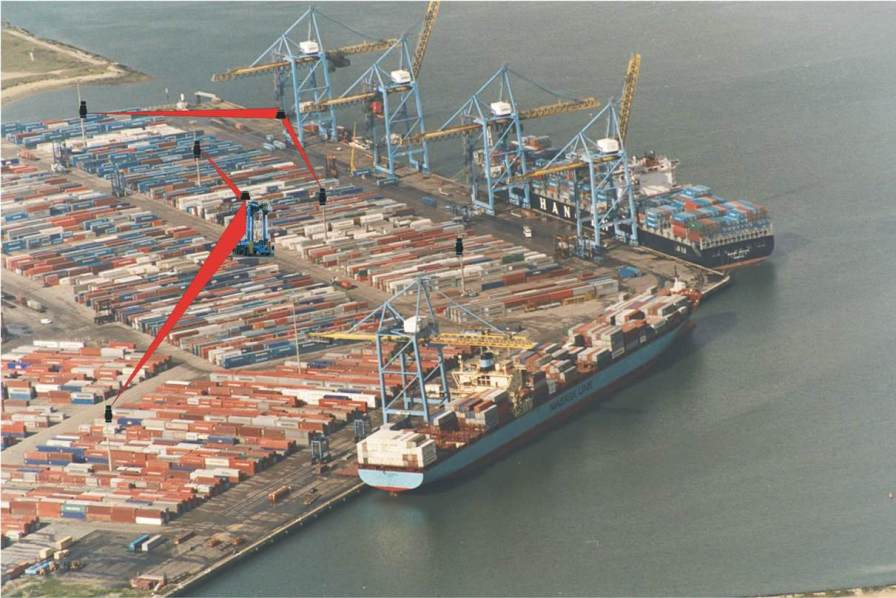
\includegraphics[width=0.6\textwidth]{./chapitres/simulation/bornesLaser.jpg}
  \caption{Réseau de bornes laser implantées sur le Terminal de Normandie (source : \href{http://www.ldtt-fr.com}{http://www.ldtt-fr.com})}
  \label{fig:bornesLaser}
\end{figure}

\begin{figure}[ht]
\centering
 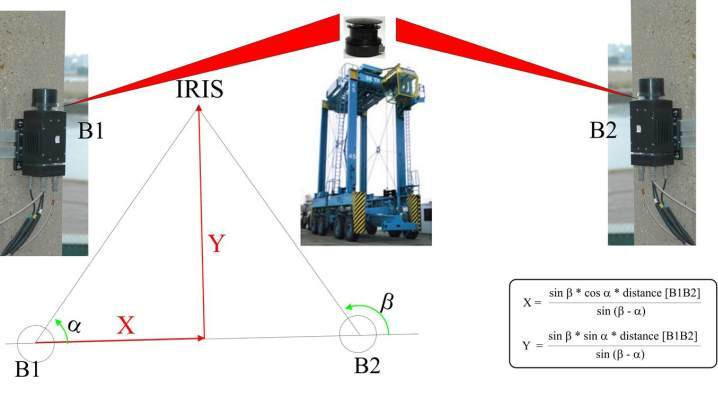
\includegraphics[width=0.6\textwidth]{./chapitres/simulation/triangularisationLaser.jpg}
  \caption{Triangularisation du signal infrarouge entre les bornes IRIS du terminal et celle d'un chariot cavalier (source : \href{http://www.ldtt-fr.com}{http://www.ldtt-fr.com})}
  \label{fig:triangularisation}
\end{figure}

Après plusieurs années de développement et de tests réels, cette technologie se montre performante et fiable et permet de connaître en temps réel la position des engins de manutention au sein du terminal. Cette information est la condition \textit{sine qua non} à toute recherche d'optimisation dynamique des activités des engins de manutention. Grâce à la position des véhicules il est ainsi possible d'optimiser dynamiquement le routage des chariots cavaliers et de prendre en compte les durées de parcours au sein du terminal. Ceci permet par conséquent, d'optimiser l'activité des chariots cavaliers tout en contrôlant le suivi de leurs opérations. En effet, lorsqu'un conteneur est chargé ou déposé par un chariot cavalier, un signal contenant la position du véhicule est envoyé au système. Ainsi, le système connaît la position de prise du conteneur (et par conséquent le conteneur chargé) ainsi que sa position de dépose. Ces informations permettent d'éviter les pertes de conteneurs au sein du terminal.

La partie LITIS du projet consistait à proposer des méthodes d'optimisation dynamique des activités des chariots cavaliers en utilisant l'information fournie par le système de géolocalisation laser. 
